\documentclass[aps,prb,reprint,superscriptaddress,floatfix,nofootinbib]{revtex4-2}

\usepackage{amsmath,amssymb,graphicx,bm,booktabs}
\usepackage[colorlinks=true,citecolor=blue,linkcolor=blue,urlcolor=blue]{hyperref}

\begin{document}

\title{Interband Pairing Signatures in the Superfluid Response of Magic-Angle Twisted Bilayer Graphene}

\author{Jian Zhou}
\affiliation{JZ Institute of Science, Hong Kong, China}
\email{jack@jzis.org}

\date{June 9, 2026}

\begin{abstract}
The large superfluid response reported in magic-angle twisted bilayer graphene
is often discussed in terms of quantum geometry, but it remains useful to ask
whether the orbital structure of the superconducting gap leaves a separable
finite-band response diagnostic.
We answer this question with an executable
Bistritzer-MacDonald--Bogoliubov-de Gennes workflow for orbital-projected
interband-pairing directions.
The pairing family is defined in the layer-sublattice basis and projected into
the normal-state band basis using a fixed time-reversal-sewn valley convention,
so that pairing direction, band projection, and response normalization can be
varied separately.
For the working direction $M_1=\tau_x\sigma_x$, the projected interband
pairing weight increases smoothly with the tuning parameter $\eta$ and reaches
approximately $0.108$ at $\eta=1$ for the $n_{\rm keep}=6$ truncation.
At fixed Frobenius norm of the orbital pairing matrix, dense scans over
chemical potential and pairing interpolation give a normalized isotropic
response change of approximately $+0.56\%$ to $+11.86\%$ between $\eta=0$ and
$\eta=1$ over $\mu=-5,\ldots,5$ meV; selected $nk=9,11,13$ checks and a
representative $nk=15$ spot check preserve the positive fixed-Frobenius sign.
The fixed raw-gap-amplitude control is much weaker and can be negative.
We therefore identify the signal as a normalization-conditioned mechanism
signature rather than an unconditional enhancement of the absolute stiffness.
An absolute-unit audit of a previous PRB-style superfluid-weight benchmark
shows that the legacy values can be only partially reconstructed from one
unified convention.
The resulting manuscript policy is that normalized response maps carry the
main mechanism claim, while absolute stiffness comparisons are deferred to a
separate benchmark calculation with a fully declared convention.
\end{abstract}

\maketitle

%====================================================================
\section{Introduction}
%====================================================================

Magic-angle twisted bilayer graphene (MATBG) provides a setting in which
superconductivity, topology, flat bands, and quantum geometry meet in a single
experimentally accessible platform~\cite{cao_sc_2018,cao_insulator_2018,yankowitz_2019}.
In conventional superconductors the superfluid weight is tied to band
dispersion and carrier density, but in flat or nearly flat bands a geometric
contribution associated with the quantum metric can remain finite even when
ordinary band velocity is small~\cite{peotta_torma_2015,torma_review_2022}.
This geometric contribution is especially relevant for MATBG, whose fragile
topology and $C_{2z}\mathcal{T}$ symmetry protect nontrivial band geometry in the
flat-band manifold~\cite{song_2019,po_2019,xie_2020_prl}.

Circuit-QED measurements have reported a superfluid stiffness in MATBG that is
large compared with a simple BCS estimate~\cite{tian_2023}.
More recent transport, microwave, and radio-frequency Josephson-junction
measurements have directly accessed superfluid stiffness or condensate
dynamics and point to nontrivial low-temperature gap
structure~\cite{tanaka_2025,portoles_2025}.
Related twisted-trilayer stiffness measurements reinforce the broader nodal-gap
phenomenology in magic-angle graphene superconductors~\cite{banerjee_2025}.
Several theoretical works have connected this anomaly to quantum geometry,
remote-band effects, and beyond-BCS corrections~\cite{hu_2019,julku_2020,verma_2021}.
Recent electron--phonon, dielectric-environment, molecular-pairing, and
strong-correlation studies further emphasize that the microscopic pairing
mechanism in twisted bilayer graphene is not yet
settled~\cite{chen_epc_2024,gao_interactions_2026,wang_molecular_pairing_2024,liang_gutzwiller_2026}.
In parallel, band-off-diagonal superconductivity has been proposed as a
candidate state in twisted graphene superlattices, and its Eliashberg
superfluid-stiffness signatures have recently been analyzed~\cite{christos_2023,putzer_2025}.
Yet a practical question remains: if a mean-field pairing ansatz contains
interband structure after projection into the MATBG band basis, does that
structure leave a robust and separable signature in the computed superfluid
response?

This paper answers that question with an explicitly executable finite-band
workflow.
Rather than starting from a band-basis off-diagonal gap chosen by hand, we
define the pairing matrix in the layer-sublattice orbital basis and project it
into the normal-state band basis.
This keeps the pairing direction covariant under band-basis gauge changes and
separates two issues that are often entangled: how interband pairing is
defined, and how the response is normalized before it is interpreted.
The main output is a normalized mechanism map,
\begin{equation}
  \delta D_{\rm iso}(\mu,\eta)
  =
  \frac{D_{\rm iso}(\mu,\eta)}
       {D_{\rm iso}(\mu,0)} - 1,
\end{equation}
computed for two gap-normalization controls.

The central result is deliberately conservative.
At fixed Frobenius norm of the orbital pairing direction, increasing the
interband-pairing component produces a reproducible change in the isotropic
response across chemical potential, with selected higher-grid checks
supporting the sign and scale of the effect.
At fixed raw gap amplitude, the effect is much smaller and sign-sensitive.
Thus the present calculation supports a normalization-conditioned mechanism
signature, not a universal statement that interband pairing always enhances
the physical superfluid stiffness.
We also perform a self-audit of the absolute units and a previous PRB-style
benchmark table; that audit sets the observable policy used below.
Normalized response ratios are the claim-bearing quantities in this mechanism
paper, whereas absolute stiffness tables should be regenerated from a single
declared convention before being used for final experimental comparison.

Figure~\ref{fig:workflow} summarizes the executable route used throughout the
paper.  The diagram is a reproducibility map rather than an additional
numerical result: it identifies where the pairing direction is defined, where
band projection enters, where the finite-band response is evaluated, and which
output is allowed to carry the mechanism claim.

\begin{figure*}[t]
\centering
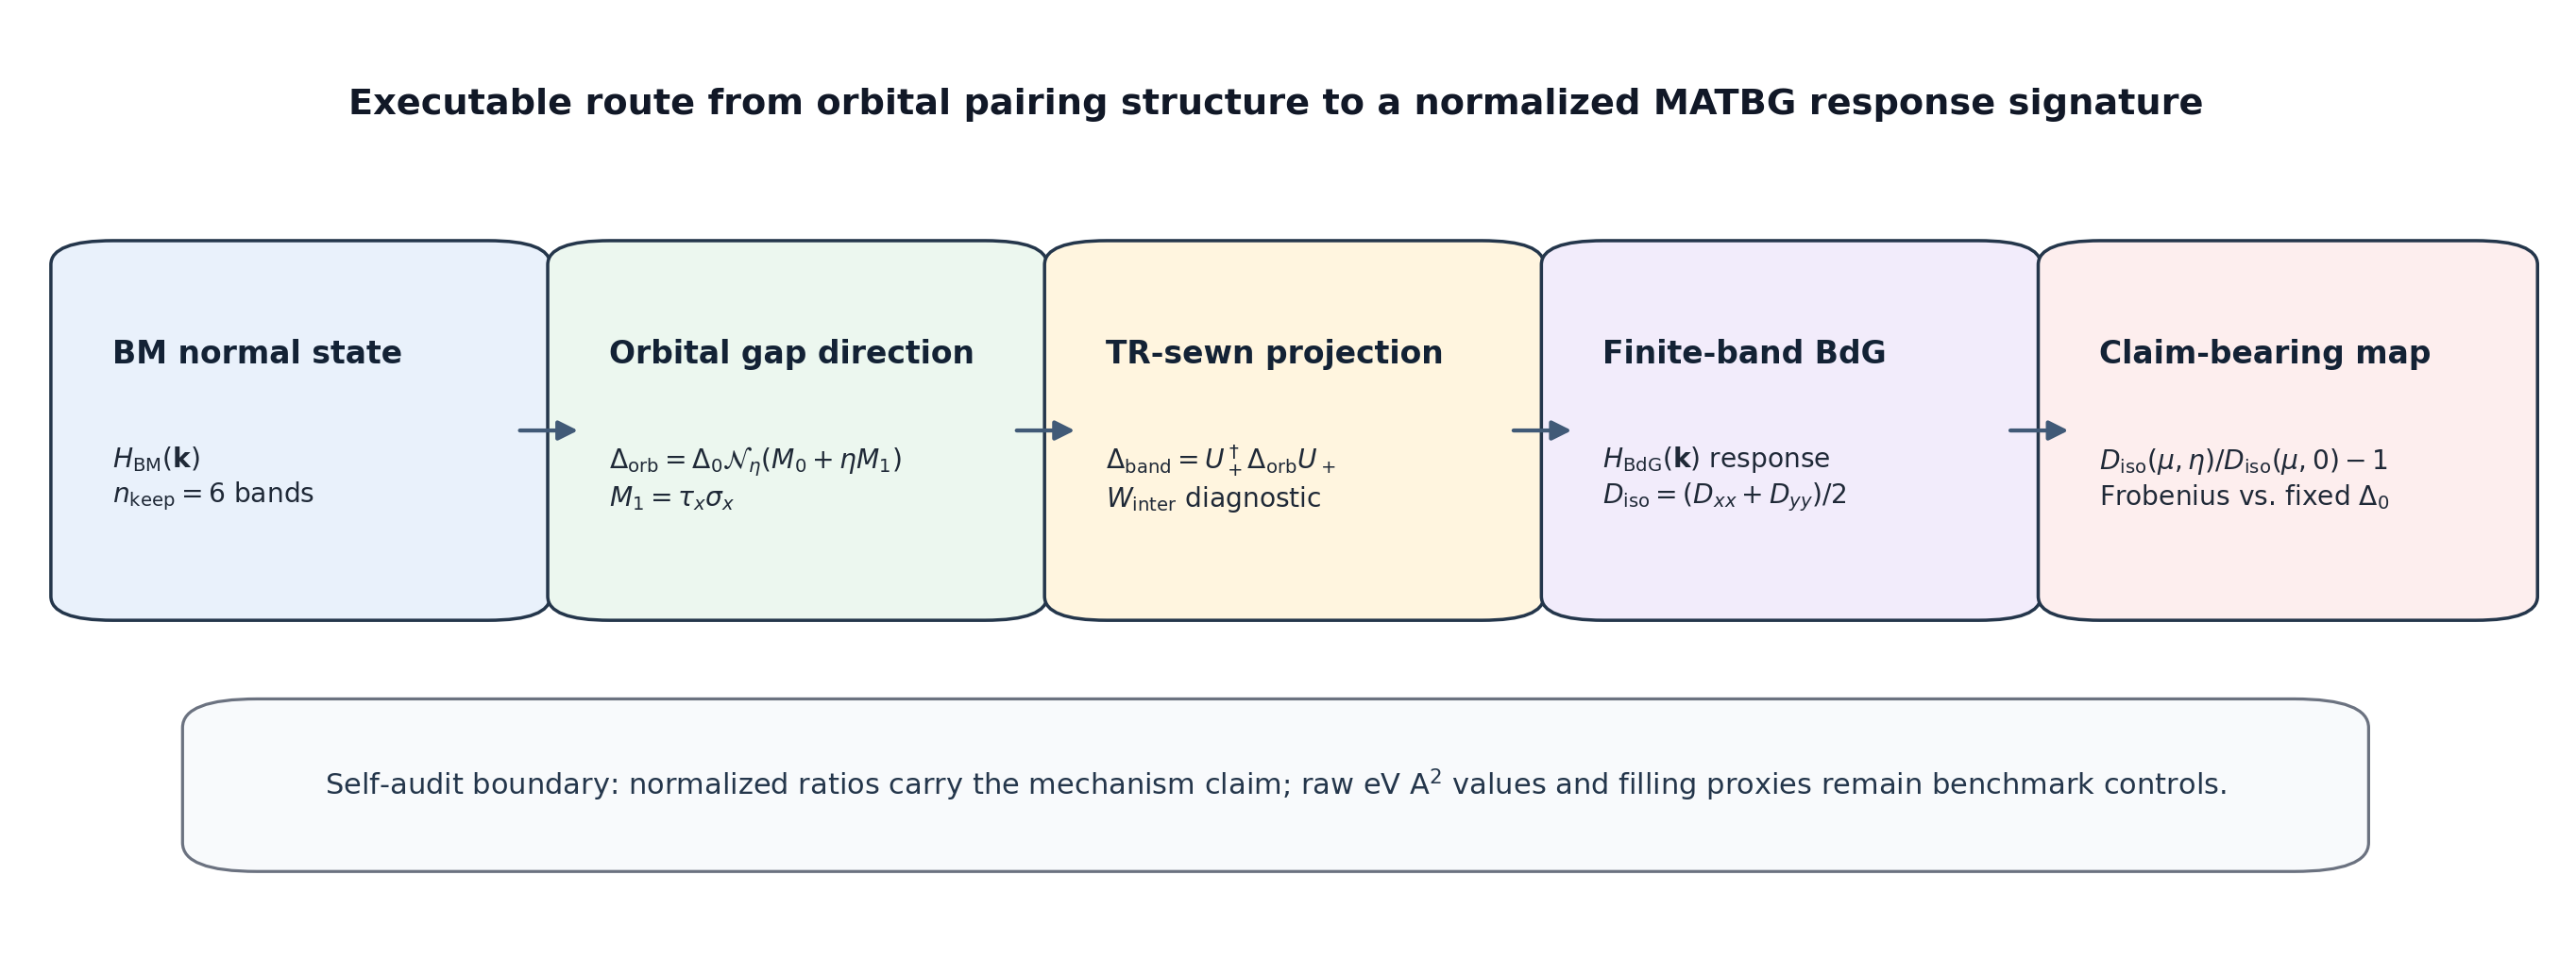
\includegraphics[width=\textwidth]{figures/workflow_schematic_prb.png}
\caption{Workflow used to convert an orbital-defined pairing direction into a
normalized finite-band response diagnostic.  The BM normal-state bands define
the retained subspace, the orbital pairing matrix is projected with the
time-reversal-sewn valley convention, the BdG response is evaluated in the
retained band space, and the claim-bearing observable is the normalized
response ratio.  Absolute eV\,\AA$^2$ values and filling proxies remain
benchmark controls in the present mechanism-paper scope.}
\label{fig:workflow}
\end{figure*}

%====================================================================
\section{Model and Pairing Construction}
%====================================================================

\subsection{Bistritzer-MacDonald model}

We use a single-valley Bistritzer-MacDonald continuum Hamiltonian with momenta
in \AA$^{-1}$ and energies in meV~\cite{bistritzer_2011}.
The basis for each moire reciprocal vector $\mathbf{G}$ is
\begin{equation}
  (tA,tB,bA,bB),
\end{equation}
where $t,b$ label top and bottom layers and $A,B$ label sublattices.
Unless otherwise stated, the numerical scans use
\begin{align}
  \theta &= 1.05^\circ, &
  v_F &= 2.135~\mathrm{eV}\,\text{\AA}, \nonumber\\
  w_0 &= 87.2~\mathrm{meV}, &
  w_1 &= 109.0~\mathrm{meV},
\end{align}
with a square reciprocal cutoff $N_{\rm shell}=3$, giving a $196\times196$
normal-state Hamiltonian per valley and spin.
The moire unit-cell area and reciprocal scale used in the unit audit are
\begin{align}
  A_M &= 1.5606\times 10^4~\text{\AA}^{2}, &
  G_M &= 0.054047~\text{\AA}^{-1}.
\end{align}

\subsection{Orbital-defined pairing family}

The pairing matrix is first specified in the orbital basis.  We write
\begin{equation}
  \Delta_{\rm orb}(\eta)
  =
  \Delta_0\,\mathcal{N}_{\eta}\left(M_0+\eta M_1\right),
\end{equation}
with
\begin{equation}
  M_0=\tau_0\sigma_0,\qquad
  M_1=\tau_x\sigma_x.
\end{equation}
Here $\tau_i$ act in layer space and $\sigma_i$ act in sublattice space.
The parameter $\eta$ interpolates between the reference orbital-singlet
direction and the interlayer-sublattice-mixed direction.
The normalization $\mathcal{N}_{\eta}$ is treated as a control variable.
We use two conventions:
\begin{align}
  &\text{fixed Frobenius:}
  &&\|M_0+\eta M_1\|_F=\|M_0\|_F,\\
  &\text{fixed }\Delta_0:
  &&\mathcal{N}_{\eta}=1.
\end{align}

At each momentum, the orbital pairing is projected into the retained band
subspace as
\begin{equation}
  \Delta_{\rm band}(\mathbf{k})
  =
  U_+^\dagger(\mathbf{k})
  \Delta_{\rm orb}
  U_-^*(-\mathbf{k}).
\end{equation}
The working valley convention is a time-reversal-sewn proxy,
$U_{-}(-\mathbf{k})=U_{+}^*(\mathbf{k})$.
Thus the production scans use
$\Delta_{\rm band}=U_+^\dagger\Delta_{\rm orb}U_+$ after the valley basis is
sewn.  A raw independently diagonalized valley-minus basis is not used for
$W_{\rm inter}$ because it is not automatically in this sewing convention.
This is used as a controlled diagnostic convention rather than a claim that all
valley-basis subtleties are solved.
The projected interband-pairing weight is
\begin{equation}
  W_{\rm inter}
  =
  \frac{\sum_{n\ne m}|\Delta_{nm}|^2}
       {\sum_{n,m}|\Delta_{nm}|^2}.
\end{equation}

%====================================================================
\section{Finite-Band Response}
%====================================================================

For each retained band subspace we construct a finite-band BdG Hamiltonian,
\begin{equation}
  H_{\rm BdG}(\mathbf{k}) =
  \begin{pmatrix}
  \varepsilon(\mathbf{k})-\mu & \Delta_{\rm band}(\mathbf{k})\\
  \Delta^\dagger_{\rm band}(\mathbf{k}) & -[\varepsilon(\mathbf{k})-\mu]
  \end{pmatrix}.
\end{equation}
The static current-current response is evaluated at zero temperature as
\begin{equation}
  \Lambda_{\alpha\beta}
  =
  \sum_{a\ne b}
  \frac{
  \langle a|J_\alpha|b\rangle
  \langle b|J_\beta|a\rangle
  (f_a-f_b)}
  {E_b-E_a}.
  \label{eq:kubo}
\end{equation}
The values reported by the executable response engine are finite-band raw
diagnostics.  They are internally consistent response outputs, but they are not
used here as final experimental stiffness values.

The band-basis velocity is decomposed into diagonal and off-diagonal parts,
\begin{equation}
  v_\alpha^{\rm band}
  =
  v_\alpha^{\rm intra}+v_\alpha^{\rm inter}.
\end{equation}
This yields conventional, geometric, and cross response channels.  The
isotropic response used in the mechanism scans is
\begin{equation}
  D_{\rm iso}=\frac{1}{2}(D_{xx}+D_{yy}).
\end{equation}
The numerical checks track BdG Hermiticity, particle-hole symmetry, and exact
closure of the channel decomposition.

%====================================================================
\section{Pairing Gates and Response Maps}
%====================================================================

\subsection{Pairing and velocity gates}

The first algebraic pairing gate verifies that an orbital-defined pairing
family transforms covariantly under band-basis gauge changes.
The BM projection gate then selects $M_1=\tau_x\sigma_x$ as a useful working
direction because it produces a finite projected interband weight in the
time-reversal-sewn valley convention while keeping $W_{\rm inter}=0$ for
$\eta=0$.
For $n_{\rm keep}=6$, $nk=7$, and $\eta=1$, the dense scan gives
\begin{equation}
  W_{\rm inter}\simeq 0.108.
\end{equation}
The velocity gate confirms that projected velocity matrices are Hermitian to
machine precision and that the intra/inter velocity split closes numerically.
These gates are not yet response claims.  They establish that the pairing
direction, valley sewing convention, and current decomposition are internally
consistent before the normalized response maps are interpreted.

\subsection{Dense chemical-potential and pairing scan}

Table~\ref{tab:dense_eta} summarizes the dense scan at $nk=7$ and
$n_{\rm keep}=6$.
It is the main endpoint comparison: each row compares $\eta=1$ with the
corresponding $\eta=0$ reference at the same chemical potential.
The fixed-Frobenius column asks how the response changes when the orbital
direction is changed at fixed matrix norm, while the fixed-$\Delta_0$ column
keeps the raw gap amplitude fixed and therefore serves as the normalization
control.
The first column gives the retained-band filling proxy $\nu_{\rm proxy}$; this
is a diagnostic occupancy proxy and is not used as a calibrated experimental
filling.  The Supplemental Material gives a central two-flat-band crosswalk;
in that convention the same chemical-potential window spans approximately
$\nu_{\rm flat}=-4$ to $+4$.
A filling-sufficiency audit verifies that this crosswalk is adequate as a BM
central-flat-band counting reference for the present mechanism maps, but not as
a device-level carrier-density calibration.

\begin{table*}[t]
\caption{Dense $\mu$ scan comparing $\eta=1$ to $\eta=0$.
The fixed-Frobenius column reports
$D_{\rm iso}(\eta=1)/D_{\rm iso}(\eta=0)-1$.
The fixed-$\Delta_0$ column reports the same quantity without rescaling the
orbital pairing matrix.
}
\label{tab:dense_eta}
\begin{ruledtabular}
\begin{tabular}{rrrr}
$\mu$ (meV) & $\nu_{\rm proxy}$ & fixed Frobenius & fixed $\Delta_0$\\
\hline
-5 & -1.483 &  0.0056 & -0.0510\\
-4 & -1.333 &  0.0891 &  0.0291\\
-3 & -1.061 &  0.0785 & -0.0071\\
-2 & -0.857 &  0.0537 & -0.0110\\
-1 & -0.653 &  0.0802 &  0.0093\\
 0 & -0.381 &  0.0817 &  0.0112\\
 1 & -0.054 &  0.0914 &  0.0044\\
 2 &  0.122 &  0.0949 &  0.0119\\
 3 &  0.395 &  0.0653 &  0.0004\\
 4 &  0.667 &  0.0662 & -0.0005\\
 5 &  0.857 &  0.1186 &  0.0312\\
\end{tabular}
\end{ruledtabular}
\end{table*}

Figure~\ref{fig:heatmap_frob} shows the fixed-Frobenius dense response map.
The table records the $\eta=1$ endpoint, while the heatmap shows how the
response evolves throughout the interpolation.
At $\eta=1$ the fixed-Frobenius response is positive for every tabulated
chemical potential, with the largest endpoint value in the present scan
occurring near $\mu=5$ meV.
The middle panel shows that the geometric fraction remains a useful diagnostic
of how the response is redistributed between current sectors.

\begin{figure*}[t]
\centering
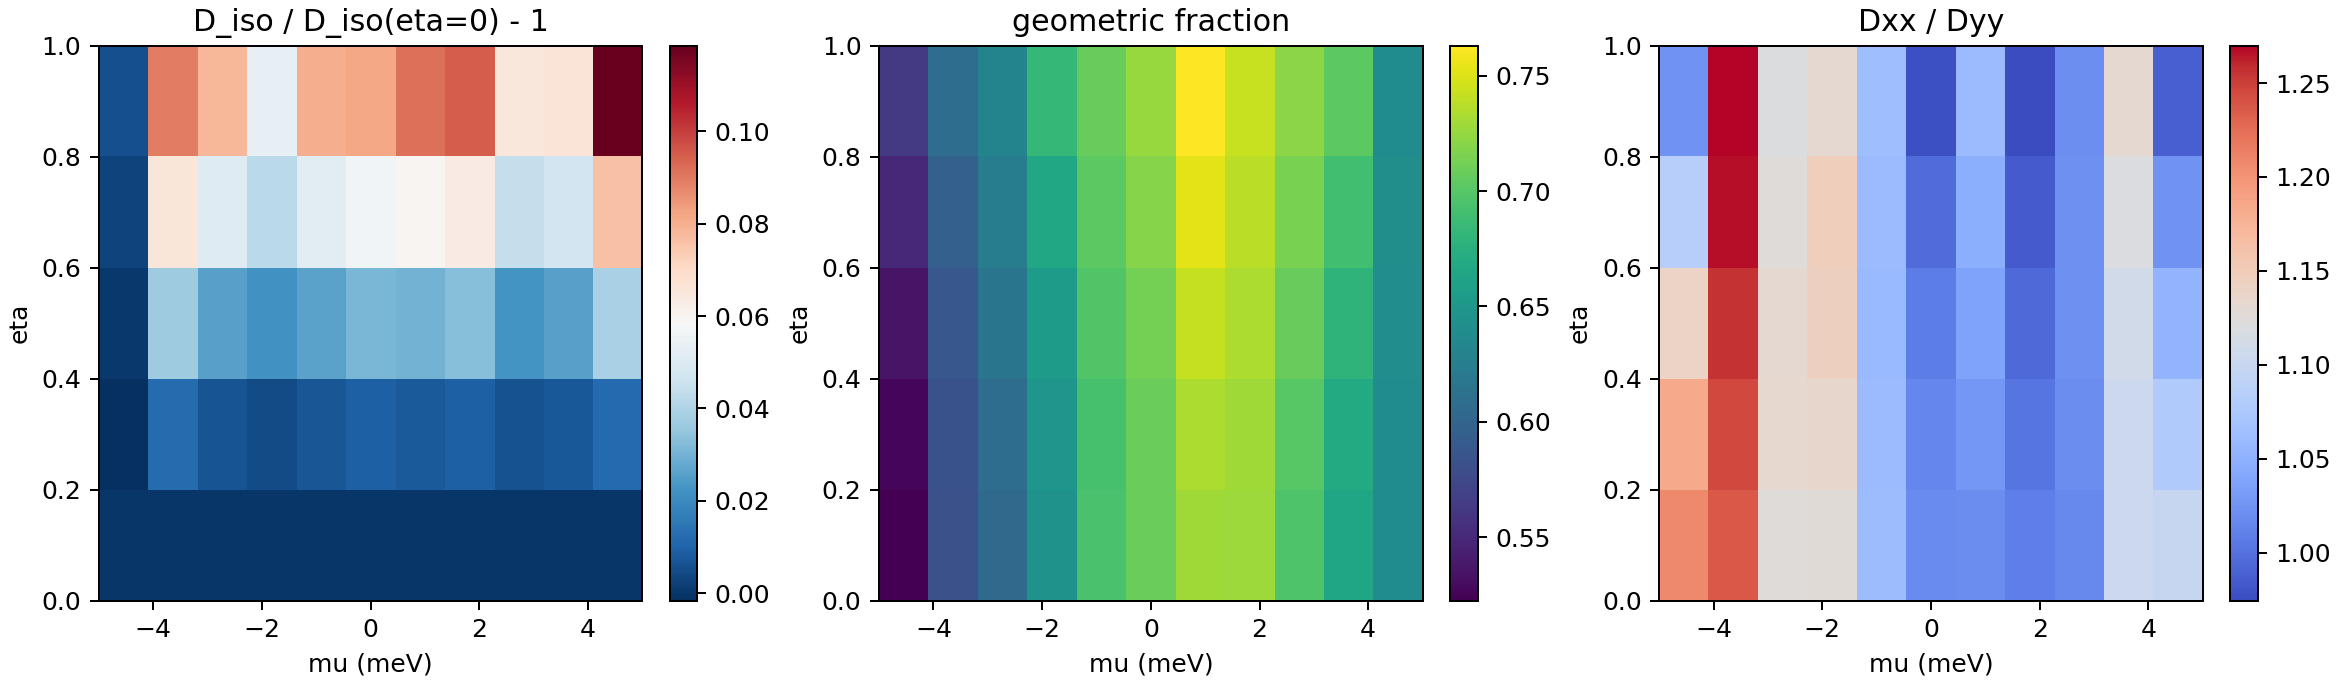
\includegraphics[width=\textwidth]{figures/mu_eta_heatmap_nk7_nkeep6_fixed_frobenius.png}
\caption{Dense $\mu$-$\eta$ response map in the fixed-Frobenius normalization.
Left: normalized isotropic response relative to $\eta=0$ at fixed $\mu$.
Middle: geometric fraction.
Right: response anisotropy $D_{xx}/D_{yy}$.
}
\label{fig:heatmap_frob}
\end{figure*}

Figure~\ref{fig:heatmap_delta0} shows the same scan at fixed raw $\Delta_0$.
The response is much weaker and can be negative.  This control is essential:
it shows that the fixed-Frobenius map should be interpreted as a response to a
specified normalized orbital direction, not as a normalization-independent
enhancement produced by any finite interband weight.

\begin{figure*}[t]
\centering
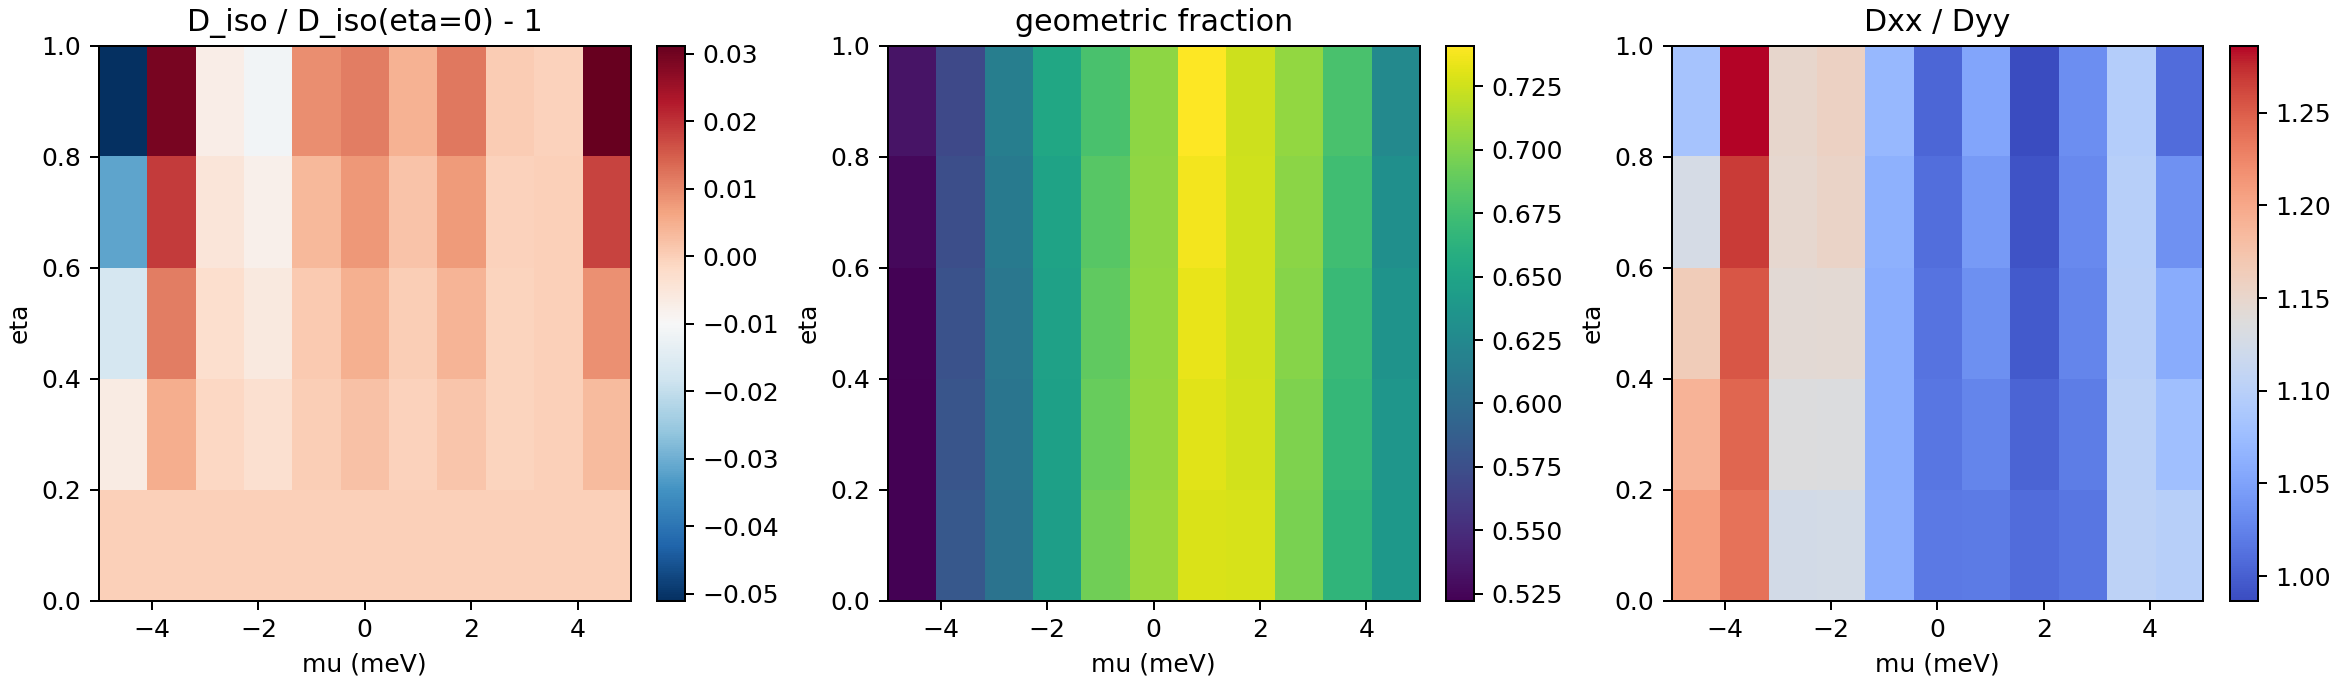
\includegraphics[width=\textwidth]{figures/mu_eta_heatmap_nk7_nkeep6_fixed_delta0.png}
\caption{Dense $\mu$-$\eta$ response map in the fixed-$\Delta_0$ normalization.
Compared with Fig.~\ref{fig:heatmap_frob}, the normalized response is strongly
suppressed and changes sign in parts of the scan.
}
\label{fig:heatmap_delta0}
\end{figure*}

\subsection{\texorpdfstring{$nk=9$}{nk=9} validation}

The key-point validation in Table~\ref{tab:nk9} repeats representative values
at $nk=9$.
It is not a replacement for the dense $nk=7$ map; rather, it tests whether the
main sign and scale survive on a finer momentum grid at chemically distinct
points.
The fixed-Frobenius signal remains positive and of comparable size, while the
fixed-$\Delta_0$ response stays close to zero.
Additional selected $nk=11$ and $nk=13$ key-point checks, reported in the
Supplemental Material, preserve the positive fixed-Frobenius response at the
same chemical potentials.
A finite-grid trend audit of these key points versus $1/nk^2$ gives positive
fixed-Frobenius intercepts between 8.65\% and 10.58\%, while the fixed-$\Delta_0$
control remains weak and sign-sensitive on the measured grids.
The Supplemental Material also reports a targeted $nk=15$ spot check at
$\mu=0$ and $2$~meV, where the fixed-Frobenius response remains +8.97\% and
+8.65\%, respectively.
A convergence-sufficiency self-audit combines these selected-grid, trend, and
spot-check data.  All audit gates pass for the selected-grid normalized
mechanism claim, while the same audit explicitly does not promote the numbers
to a strict continuum-limit value.

\begin{table}[t]
\caption{$nk=9$, $n_{\rm keep}=6$ validation of the $\eta=1$ response.}
\label{tab:nk9}
\begin{ruledtabular}
\begin{tabular}{rrr}
$\mu$ (meV) & fixed Frobenius & fixed $\Delta_0$\\
\hline
-4 & 0.0604 & -0.0068\\
 0 & 0.0863 &  0.0103\\
 2 & 0.0643 & -0.0029\\
 4 & 0.0605 & -0.0017\\
\end{tabular}
\end{ruledtabular}
\end{table}

%====================================================================
\section{Self-Audit of Absolute Units}
%====================================================================

The raw response engine outputs values in finite-band diagnostic units.
A conservative conversion maps raw meV\,\AA$^2$ to eV\,\AA$^2$ per flavor by
dividing by $1000$.
Any spin/valley degeneracy factor is left outside this conversion:
\begin{equation}
  D_{\rm per~flavor}[\mathrm{eV}\,\text{\AA}^2]
  =
  D_{\rm raw}[\mathrm{meV}\,\text{\AA}^2]/1000.
\end{equation}
The moire area and reciprocal scale agree with the standard MATBG geometry,
but the prior band-basis decomposition benchmark table~\cite{zhou_decomposition_2026}
is not reproduced by a single global prefactor or by the present production
convention.
The claim-bearing observable policy for the present manuscript is therefore:
the production $\tau_z/\tau_0$ finite-band response convention is used for
normalized ratios and channel diagnostics, while eV\,\AA$^2$ per-flavor values
are restricted to benchmark provenance and self-audit tables.

Table~\ref{tab:prb_audit} summarizes the reconstruction audit for uniform
$s$-wave pairing at $\mu=0$, $\Delta_0=1$ meV, and $nk=14$.
The best simple unified reconstruction is
\begin{equation}
  D_{\rm conv}=2D_{\rm intra,\tau_z},\qquad
  D_{\rm geom}=D_{\rm inter,\tau_z}.
\end{equation}
It nearly reconstructs the extended-band endpoint but not the flat-band
endpoint.
A separate flat-band audit shows that the old $n_{\rm keep}=2$ total and
conventional values can be approximated with a Gamma-centered mesh and a full
curvature-like conventional correction, but that correction does not work
cleanly at $n_{\rm keep}=6$.

\begin{table*}[t]
\caption{Prior band-basis benchmark reconstruction.
Values are eV\,\AA$^2$ per flavor.  The reconstruction route is kept separate
from the production interband-pairing scans.
}
\label{tab:prb_audit}
\begin{ruledtabular}
\begin{tabular}{lrrrrrr}
case & $n_{\rm keep}$ & $D_{\rm total}$ & target & $D_{\rm conv}$ & target & $D_{\rm geom}$\\
\hline
current $\tau_z/\tau_0$ & 2 & 29.34 & 67.50 & 20.95 & 53.00 & 8.40\\
double-conv all-$\tau_z$ & 2 & 54.40 & 67.50 & 41.89 & 53.00 & 12.50\\
flat endpoint audit & 2 & 66.18 & 67.50 & 53.83 & 53.00 & 12.36\\
double-conv all-$\tau_z$ & 6 & 126.66 & 129.30 & 51.45 & 54.00 & 75.22\\
\end{tabular}
\end{ruledtabular}
\end{table*}

This self-audit changes the interpretation of absolute stiffness values.
The historical table is useful as a benchmark, but it should not be used to
set the convention for the present interband-pairing mechanism scans.
If a later version adds direct experimental comparison, absolute tables should
be regenerated from one declared response convention, with degeneracy,
Brillouin-zone normalization, and any diamagnetic or curvature term stated
explicitly.

%====================================================================
\section{Discussion}
%====================================================================

The main physical message is that an interband-pairing direction can leave a
detectable imprint on the normalized finite-band response of MATBG.
The imprint is reproducible across chemical potential and survives a modest
increase of the momentum grid, but it depends strongly on how the orbital gap
direction is normalized.
This is both a result and a warning: interband pairing is not a scalar knob.
Changing the orbital structure can also change the total norm of the projected
gap, and the resulting response should not be interpreted without specifying
the normalization convention.

The self-audit also clarifies the status of absolute stiffness claims.
The continuum BM model has subtleties associated with UV regularization,
current convention, and band truncation.  Those subtleties are manageable, but
the audit shows that old absolute tables can mix conventions in ways that are
not captured by one simple prefactor.
For this reason the most robust near-term observable in the present work is a
normalized response map, not an absolute stiffness prediction.
Likewise, $\nu_{\rm proxy}$ in the tables is a retained-band occupancy proxy
defined for scan organization, not a calibrated carrier density.  The
Supplemental Material gives a central two-flat-band filling crosswalk for the
dense scan, but the present figures should still be read as functions of
chemical potential and retained-band occupancy, not as a quantitative map onto
an experimental superconducting dome.
Within that restricted use, the filling-sufficiency audit shows that the dense
scan spans the full central two-flat-band counting range and samples reference
points near $\nu_{\rm flat}=0$ and $\pm2$.
The Supplemental Material also includes a claim-scope audit that separates the
allowed normalized-response mechanism claims from deferred absolute-stiffness,
device-calibration, and continuum-limit claims.

The evidence chain is therefore intentionally narrower than a full
microscopic theory of MATBG superconductivity.
The pairing gates establish that the orbital construction creates a finite
band-off-diagonal component after projection; the dense maps show that this
component changes the normalized response when the orbital pairing direction is
compared at fixed Frobenius norm; the fixed-$\Delta_0$ maps show that the same
statement is not normalization independent; and the selected-grid audits test
that the sign and scale are not artifacts of the smallest momentum grid.
The interpretation would be weakened if the projected interband weight became
unstable under the retained-band or grid choices, if the fixed-Frobenius signal
lost its sign stability on the selected higher grids, or if the fixed-$\Delta_0$
control showed the same response pattern.
None of these checks replaces a self-consistent pairing calculation, but they
make the present conclusion falsifiable within the finite-band diagnostic
framework used here.

Several limitations remain.  First, the valley sewing convention used here is a
controlled time-reversal proxy; a fully independent two-valley implementation
would be required for valley-asymmetric perturbations or final absolute
production calculations.
Second, a direct experimental-comparison version would require a final absolute
response convention; the present mechanism paper therefore makes no
claim-bearing absolute stiffness prediction.  Third, the filling variable is
currently a retained-band occupancy proxy.  Fourth, no self-consistent gap
equation is solved.  Fifth, a UV-complete lattice calculation would be required
for final quantitative comparison with experiment.
Recent direct imaging of interaction-reshaped flat bands in MATBG also
suggests that a future quantitative comparison should revisit the normal-state
band structure beyond the noninteracting BM spectrum used here~\cite{xiao_flat_bands_2026}.
Finally, the present ansatz is deliberately simpler than recent microscopic
band-off-diagonal and finite-momentum scenarios.  Recent tunneling and STM
work in magic-angle graphene reports nodal-gap, separated-gap, and intervalley
features, while theory has connected band-off-diagonal and Kekul\'e
pair-density-wave structures to spectral and stiffness
signatures~\cite{park_nodal_gap_2025,kim_intervalley_2026,christos_2023,putzer_2025,wang_levin_kekule_2026,wang_kekule_2026}.
Those states are complementary to the present uniform orbital-projected
diagnostic and will require a separate finite-momentum BdG extension.

%====================================================================
\section{Conclusions}
%====================================================================

The calculation isolates a concrete finite-band diagnostic of pairing
structure in MATBG.
For the orbital direction $M_1=\tau_x\sigma_x$, the projected interband weight
is finite and the fixed-Frobenius response map shows a reproducible positive
change across the scanned chemical-potential window.
The fixed-$\Delta_0$ control, by contrast, is weak and sign-sensitive.
This contrast is the central result: interband pairing produces a
normalization-conditioned mechanism signature in the finite-band MATBG
superfluid response, not an absolute stiffness prediction independent of how
the gap direction is normalized.

The self-audit of units and filling fixes the scope of this conclusion.
Normalized response ratios are robust claim-bearing observables for the
present mechanism paper, while absolute stiffness tables, device-level filling
calibration, and continuum-limit extrapolation remain separate tasks.
Within that boundary, the work provides an executable route for comparing
orbital gap structure, band projection, and quantum-geometric response in
magic-angle graphene superconductivity, together with explicit checks that can
invalidate or sharpen the mechanism claim in future higher-fidelity
calculations.

\begin{acknowledgments}
The author acknowledges use of open-source scientific computing tools
including NumPy and Matplotlib.
\end{acknowledgments}

\section*{Declarations}

\textbf{Funding}: Not applicable.

\textbf{Conflict of interest}: The author declares no conflict of interest.

\textbf{Data availability}: All data and code supporting this work are available
from the corresponding author upon reasonable request.

\textbf{Ethics approval}: Not applicable.

\bibliography{references}

\end{document}
